\documentclass[12pt]{article}

	\usepackage{answers}
	\usepackage{float}
	\usepackage{setspace}
	\usepackage{graphicx}
	\usepackage{enumitem}
	\usepackage{multicol}
	\usepackage{mathrsfs}
	\usepackage{listings}
	\lstset{basicstyle=\ttfamily\footnotesize}
	\usepackage[margin=1in]{geometry} 
	\usepackage{amsmath,amsthm,amssymb}
	 
	\usepackage[margin=-1cm]{caption}
	 
	\newcommand{\N}{\mathbb{N}}
	\newcommand{\Z}{\mathbb{Z}}
	\newcommand{\C}{\mathbb{C}}
	\newcommand{\R}{\mathbb{R}}
	
	\DeclareMathOperator{\sech}{sech}
	\DeclareMathOperator{\csch}{csch}
	 
	\newenvironment{theorem}[2][Theorem]{\begin{trivlist}
	\item[\hskip \labelsep {\bfseries #1}\hskip \labelsep {\bfseries #2.}]}{\end{trivlist}}
	\newenvironment{definition}[2][Definition]{\begin{trivlist}
	\item[\hskip \labelsep {\bfseries #1}\hskip \labelsep {\bfseries #2.}]}{\end{trivlist}}
	\newenvironment{proposition}[2][Proposition]{\begin{trivlist}
	\item[\hskip \labelsep {\bfseries #1}\hskip \labelsep {\bfseries #2.}]}{\end{trivlist}}
	\newenvironment{lemma}[2][Lemma]{\begin{trivlist}
	\item[\hskip \labelsep {\bfseries #1}\hskip \labelsep {\bfseries #2.}]}{\end{trivlist}}
	\newenvironment{exercise}[2][Exercise]{\begin{trivlist}
	\item[\hskip \labelsep {\bfseries #1}\hskip \labelsep {\bfseries #2.}]}{\end{trivlist}}
	\newenvironment{solution}[2][Solution]{\begin{trivlist}
	\item[\hskip \labelsep {\bfseries #1}]}{\end{trivlist}}
	\newenvironment{problem}[2][Problem]{\begin{trivlist}
	\item[\hskip \labelsep {\bfseries #1}\hskip \labelsep {\bfseries #2.}]}{\end{trivlist}}
	\newenvironment{question}[2][Question]{\begin{trivlist}
	\item[\hskip \labelsep {\bfseries #1}\hskip \labelsep {\bfseries #2.}]}{\end{trivlist}}
	\newenvironment{corollary}[2][Corollary]{\begin{trivlist}
	\item[\hskip \labelsep {\bfseries #1}\hskip \labelsep {\bfseries #2.}]}{\end{trivlist}}
	 
	\begin{document}
	 
	% --------------------------------------------------------------
	%                         Start here
	% --------------------------------------------------------------
	 
	\title{Homework 4}%replace with the appropriate homework number
	\author{Christian Steinmetz\\ %replace with your name
	MATH 8090-Spring 2018} %if necessary, replace with your course title
	 
	\maketitle
	
	\begin{problem}{6}
	$ $ \\
	$ $ \\
	Consider the data set of global marine temperatures (yearly data) in globaltmpmarine.txt (on blackboard). Find the best fitting time series model using diagnostics, parsimony and selection criteria (like BIC).  Consider models with and without trend parameters.  Decide if the trend is statistically significant. Use your fitted model to forecast the next three values. Write a short report describing your model fitting experience. Be sure to include
	\begin{enumerate}[label=(\alph*)]
		\item An overview of your model fitting process
		\item Any plots you used to decide on a model.
		\item A list of candidate models considered.
		\item A summary of results for the various models fit to the data (like a table containing BIC values for example)
		\item A complete description of your final model.
		\item A plot showing the time series and three forecasts with approximate 95\% prediction intervals.
	\end{enumerate}
	
	\end{problem}
	
	\begin{solution}{}
	$ $ \\
	$ $ \\
	A plot of the original data is shown below in Figure \ref{fig:temp_data}. We can argue that there is an upward trend in the data that may be fit with a linear or quadratic trend. \\

	
	First we fit a linear trend and then plot the ACF and PACF of the residuals which are shown in Figure \ref{fig:temp_acf} and Figure \ref{fig:temp_pacf}. From the ACF we see significant autocorrelation at lag $1$ and lag $4$. The PACF shows no significant autocorrelation for $h > 1$. This suggests that an AR(1) or AR(4) with linear trend may be an appropriate model. 
		
	\begin{figure}[H]
    		\centering
    		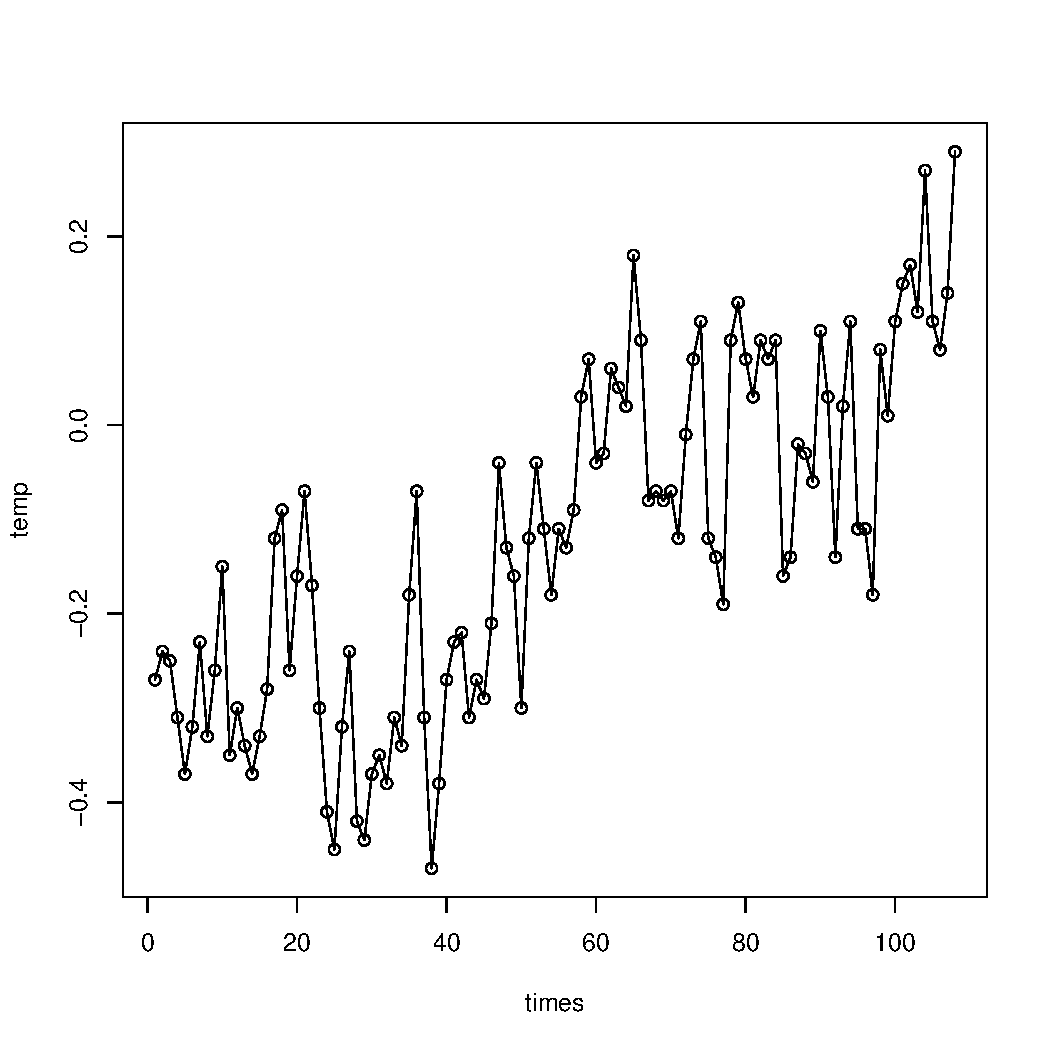
\includegraphics[width=0.5\textwidth]{figs/problem_6/temp_data.pdf}
    		\caption{Global martime temperature data.}
    		\label{fig:temp_data}
	\end{figure}
	
	\begin{figure}[H]
    		\centering
    		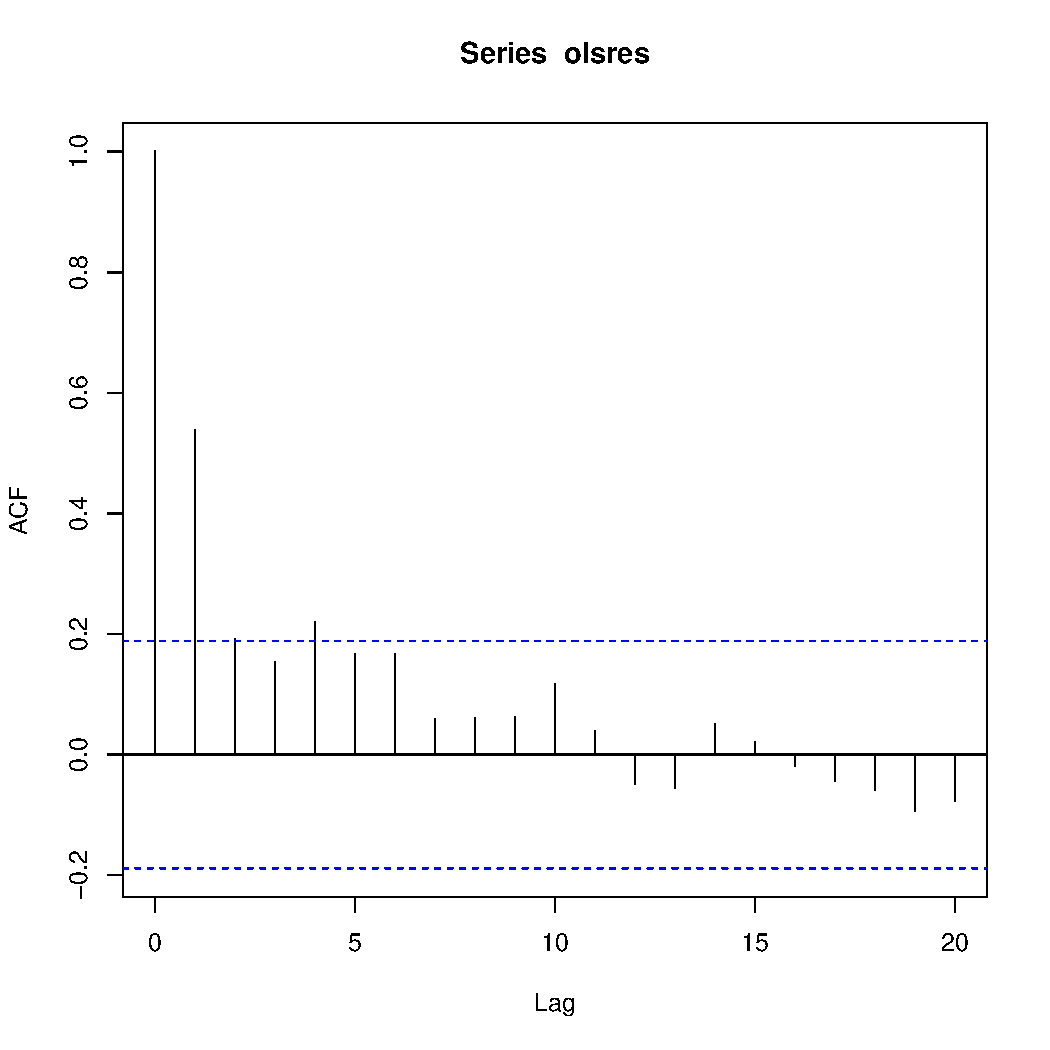
\includegraphics[width=0.5\textwidth]{figs/problem_6/temp_acf.pdf}
    		\caption{ACF of residuals from linear fit.}
    		\label{fig:temp_acf}
	\end{figure}
	
	\begin{figure}[H]
    		\centering
    		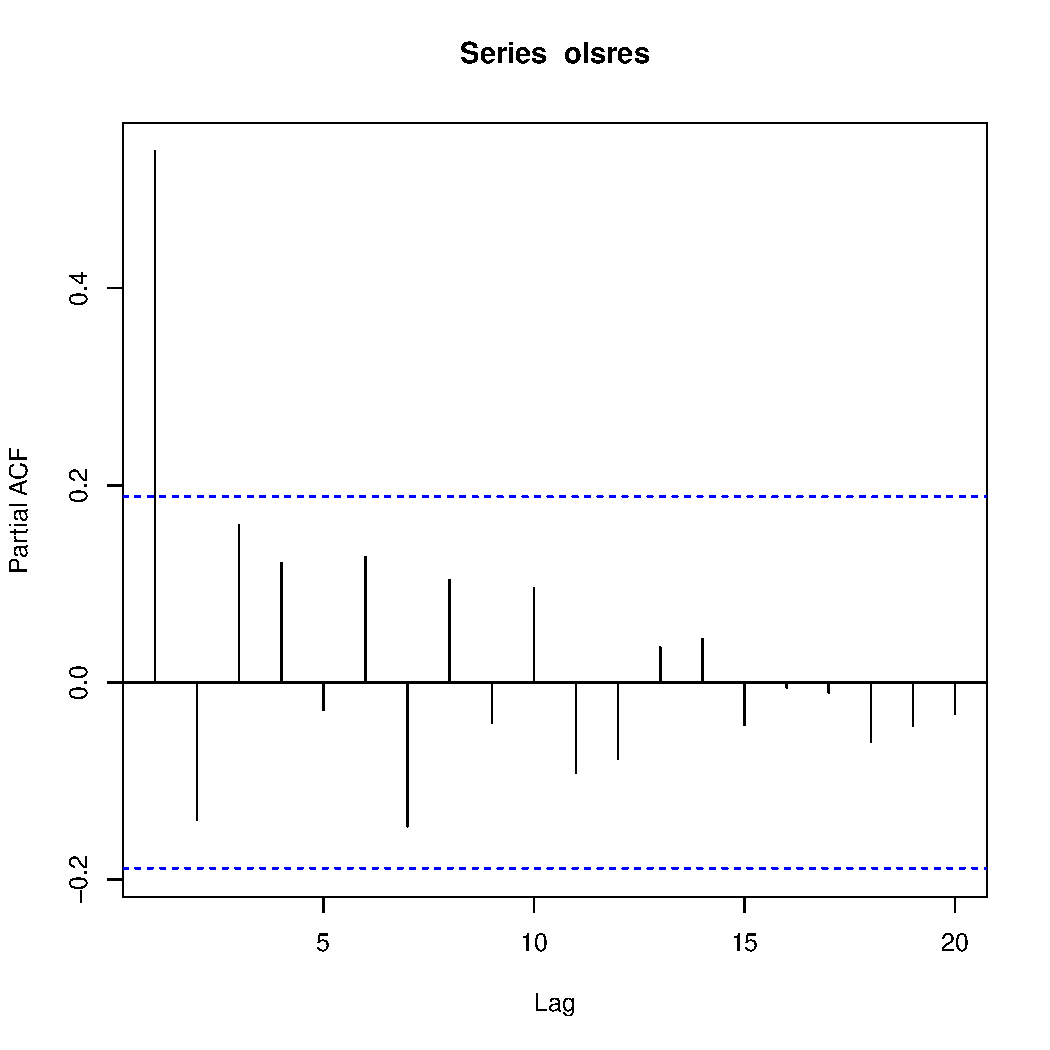
\includegraphics[width=0.5\textwidth]{figs/problem_6/temp_pacf.pdf}
    		\caption{PACF of residuals from linear fit.}
    		\label{fig:temp_pacf}
	\end{figure}
	

	Our linear trend with AR(1) errors is shown in Figure \ref{fig:temp_ar1_lin} and is followed by  our linear trend with AR(4) errors shown in Figure \ref{fig:temp_ar4_lin}.

	\begin{figure}[H]
    		\centering
    		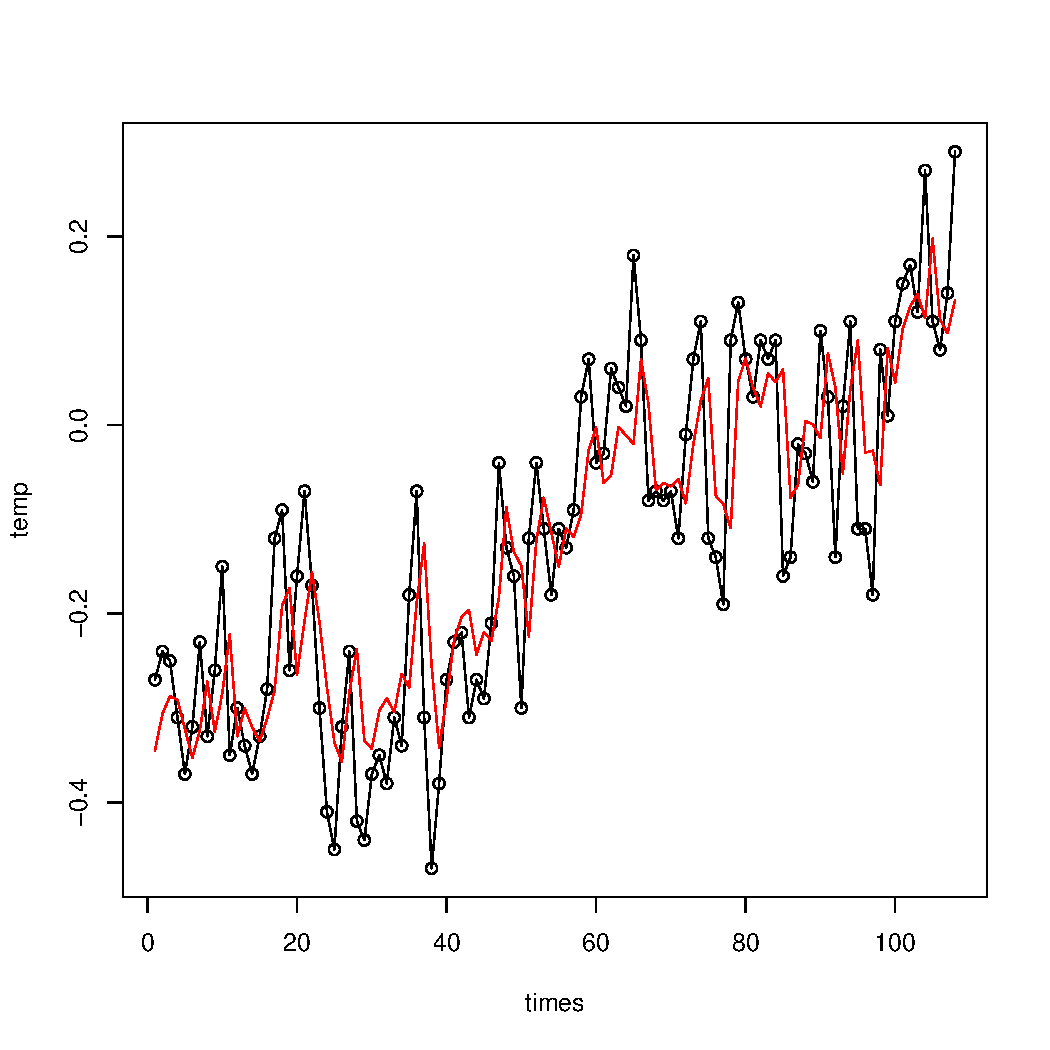
\includegraphics[width=0.6\textwidth]{figs/problem_6/temp_ar1_lin.pdf}
    		\caption{AR(1) fit with linear trend.}
    		\label{fig:temp_ar1_lin}
	\end{figure}
	
	\begin{lstlisting}
Coefficients:
        ar1  intercept   times
      0.550    -0.3645  0.0045
s.e.  0.081     0.0391  0.0006

sigma^2 estimated as 0.008728:  log likelihood = 102.6,  aic = -197.2
[BIC] -186.4743

        Box-Ljung test

data:  ar1fit$resid
X-squared = 16.053, df = 15, p-value = 0.3785
	\end{lstlisting}
	
	\begin{figure}[H]
    		\centering
    		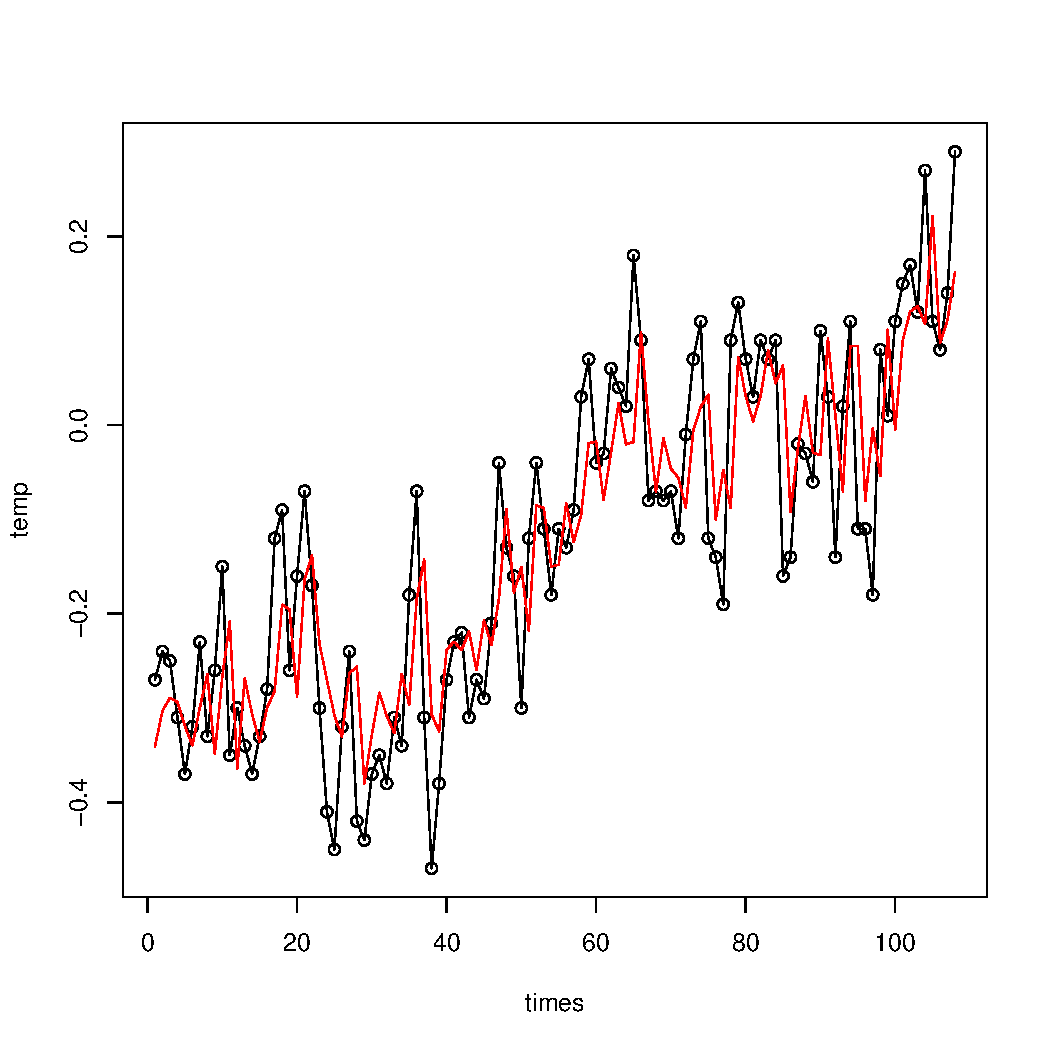
\includegraphics[width=0.6\textwidth]{figs/problem_6/temp_ar4_lin.pdf}
    		\caption{AR(4) fit with linear trend.}
    		\label{fig:temp_ar4_lin}
	\end{figure}
	
	
		\begin{lstlisting}
Coefficients:
         ar1      ar2     ar3     ar4  intercept   times
      0.6342  -0.2199  0.0861  0.1223    -0.3619  0.0044
s.e.  0.0963   0.1134  0.1133  0.0956     0.0440  0.0007

sigma^2 estimated as 0.008174:  log likelihood = 106.05,  aic = -198.1
[BIC] -179.3265

        Box-Ljung test

data:  ar4fit$resid
X-squared = 9.2165, df = 15, p-value = 0.8659
	\end{lstlisting}
	
	From the p-values of the Box-Ljung tests we can show that both models are adequate. We also attempt to fit a model without a linear trend using differencing. The results for the ARIMA(1,1,0), ARIMA(4,1,0), and ARIMA(4,1,1) are shown below.	
	
	\begin{lstlisting}
Coefficients:
          ar1
      -0.1069
s.e.   0.0966

sigma^2 estimated as 0.01113:  log likelihood = 88.84,  aic = -173.67
[BIC] -168.3287

        Box-Ljung test
X-squared = 34.807, df = 23, p-value = 0.05436
	
	\end{lstlisting}	

	\begin{lstlisting}
Coefficients:
         ar1      ar2      ar3      ar4
      -0.251  -0.4202  -0.2560  -0.0756
s.e.   0.097   0.0965   0.0963   0.0968

sigma^2 estimated as 0.0091:  log likelihood = 99.36,  aic = -188.71
[BIC] -175.3473

        Box-Ljung test
X-squared = 16.85, df = 23, p-value = 0.8165
	\end{lstlisting}
	
	
	\begin{lstlisting}
	Coefficients:
         ar1      ar2     ar3     ar4      ma1
      0.4958  -0.2587  0.0309  0.0679  -0.7844
s.e.  0.2081   0.1211  0.1329  0.1252   0.1836

sigma^2 estimated as 0.008849:  log likelihood = 100.77,  aic = -189.54
[BIC] -173.5042

        Box-Ljung test
X-squared = 13.941, df = 23, p-value = 0.9286	
        \end{lstlisting}


	All four models were found to be adequate and based upon our AIC and BIC values shown in the table below we select the AR(1) model since it had the smallest BIC even though some of the larger models have a higher AIC, although the AIC tends to overfit and does not take into account the number of model parameters. 
	
	\begin{center}
	\begin{tabular}{ |c|c|c| } 
	\hline
	Model & AIC & BIC \\
	\hline
 	AR(1) & -197.2 & -186.4743 \\ 
 	AR(4) & -198.1 & -179.3265 \\ 
	ARIMA(4,0,1) & -200.8 & -179.3456 \\
 	ARIMA(1,1,0) & -173.67 & -168.3287 \\ 
	ARIMA(4,1,0) & -188.71 & -175.3473 \\ 
	ARIMA(4,1,1) & -189.54 & -173.5042 \\
 	\hline
	\end{tabular}
	\end{center}

	\newpage

	The AR(1) form is as follows
	
	\begin{equation*}
	X_t = \mu + \phi_1 X_{t-1} + Z_t,
	\end{equation*}
	
	\begin{equation*}
	\{Z_t\} \sim \text{WN}(0,\sigma^2).
	\end{equation*}
	
	The fitted AR(1) with linear regression term is given by 
	
	\begin{equation*}
	X_t = -0.3645 + 0.0045t +0.550 X_{t-1} + Z_t,
	\end{equation*}
	
	\begin{equation*}
	\{Z_t\} \sim \text{WN}(0,\sigma^2).
	\end{equation*}
	
	 
	Predicting three time steps ahead produces the following results with the associated 95\% confidence intervals shown in Figure \ref{fig:temp_pred}.
	
	
	\begin{figure}[H]
    		\centering
    		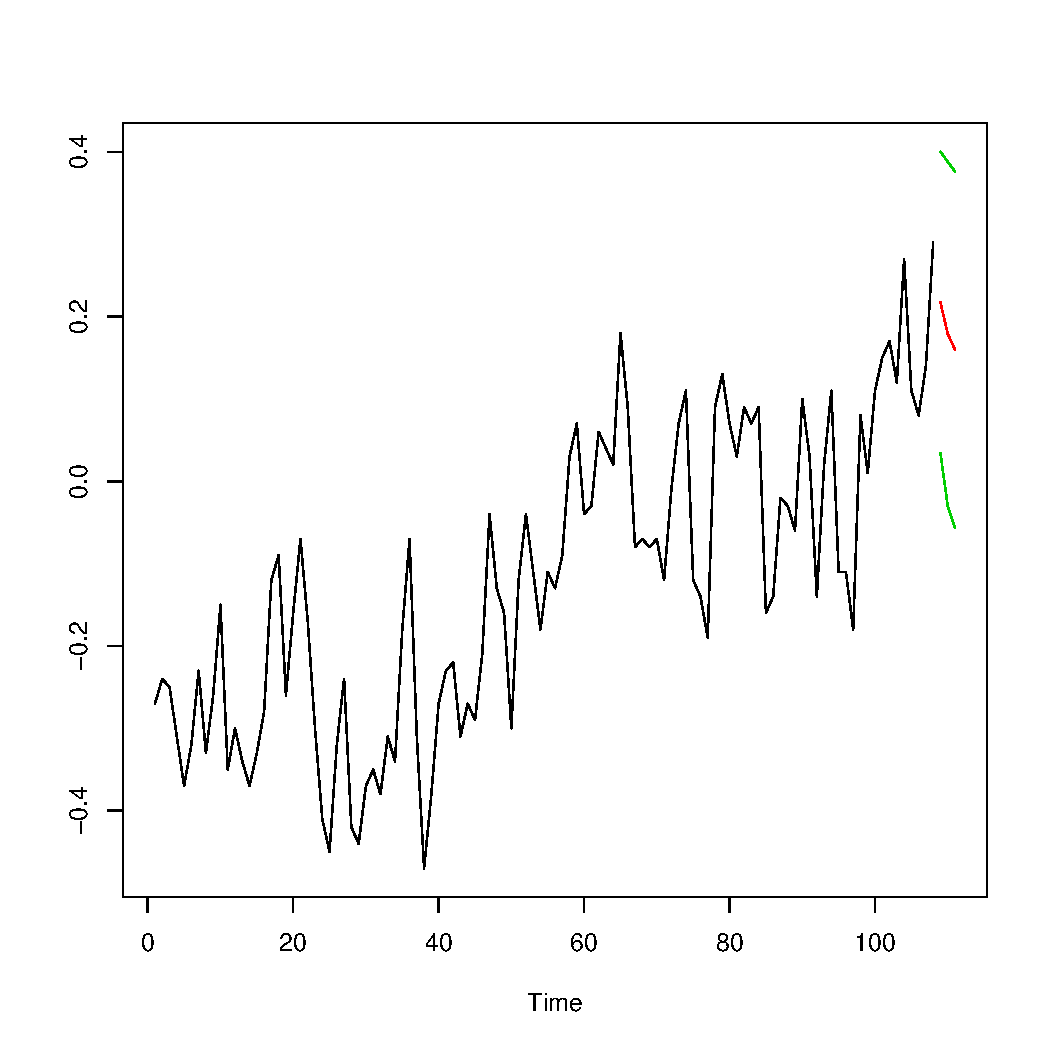
\includegraphics[width=0.8\textwidth]{figs/problem_6/temp_arima_pred.pdf}
    		\caption{Three step ahead prediction using linear fit with AR(1) errors.}
    		\label{fig:temp_pred}
	\end{figure}
	
	\newpage
	\end{solution}

	\newpage
	
	\begin{problem}{8}
	$ $ \\
	$ $ \\
	Consider the airline data modeled in class (see R code on Canvas).  We will assess the predictive ability of time series models for this data as follows.  Use the first ten years of data: Y1,\ldots,Y120 to 
	\begin{enumerate}[label=(\alph*)]
		\item Find the best fitting time series regression model you can find for the log(y) values.
		\item Find the best fitting SARIMA model for the first 10 years of data.
		\item	Use each model to forecast the last year of data and compare your total forecast error for the two models.  Which 	model has smaller error?  Which model has smaller AICC? 
		\item	Use the fitted model to show how the forecast at time 121 is calculated using each of your model fits.    
	\end{enumerate}
	\end{problem}
		
	\begin{solution}{}
	$ $ \\
	$ $ \\
	\begin{enumerate}[label=(\alph*)]
		\item We start with the AR(1) model and monthly dummy variables to account for the periodic trend. In addition we fit an AR(2) with the same monthly dummy variables since the ACF plot suggests there me be correlation beyond lag 1. It was found that adding further autoregression parameters did not improve the AIC or BIC values of the model. Using the Box-Ljung test we find no evidence of significant autocorrelation in the residuals of the fitted models so we can say both the AR(1) and AR(2) are adequate. We actually find that the AR(2) fit has a slightly greater AIC and BIC value. There the AR(1) model was chosen since it had both the smallest AIC and BIC values and also employed the least amount of parameters. 
		
	\begin{figure}[H]
    		\centering
    		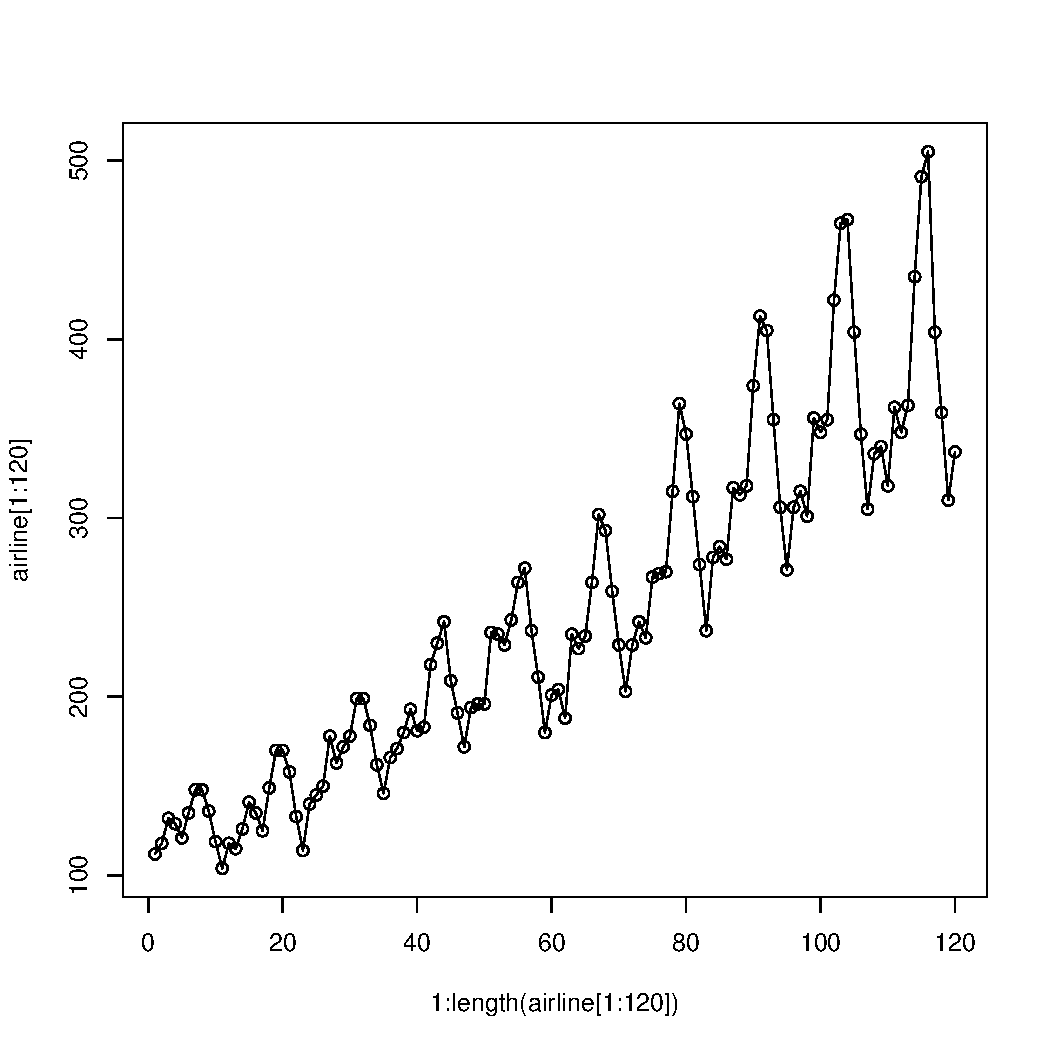
\includegraphics[width=0.6\textwidth]{figs/problem_8/airline.pdf}
    		\caption{First ten years of monthly airline data.}
    		\label{fig:airline}
	\end{figure}
	
	\begin{figure}[H]
    		\centering
    		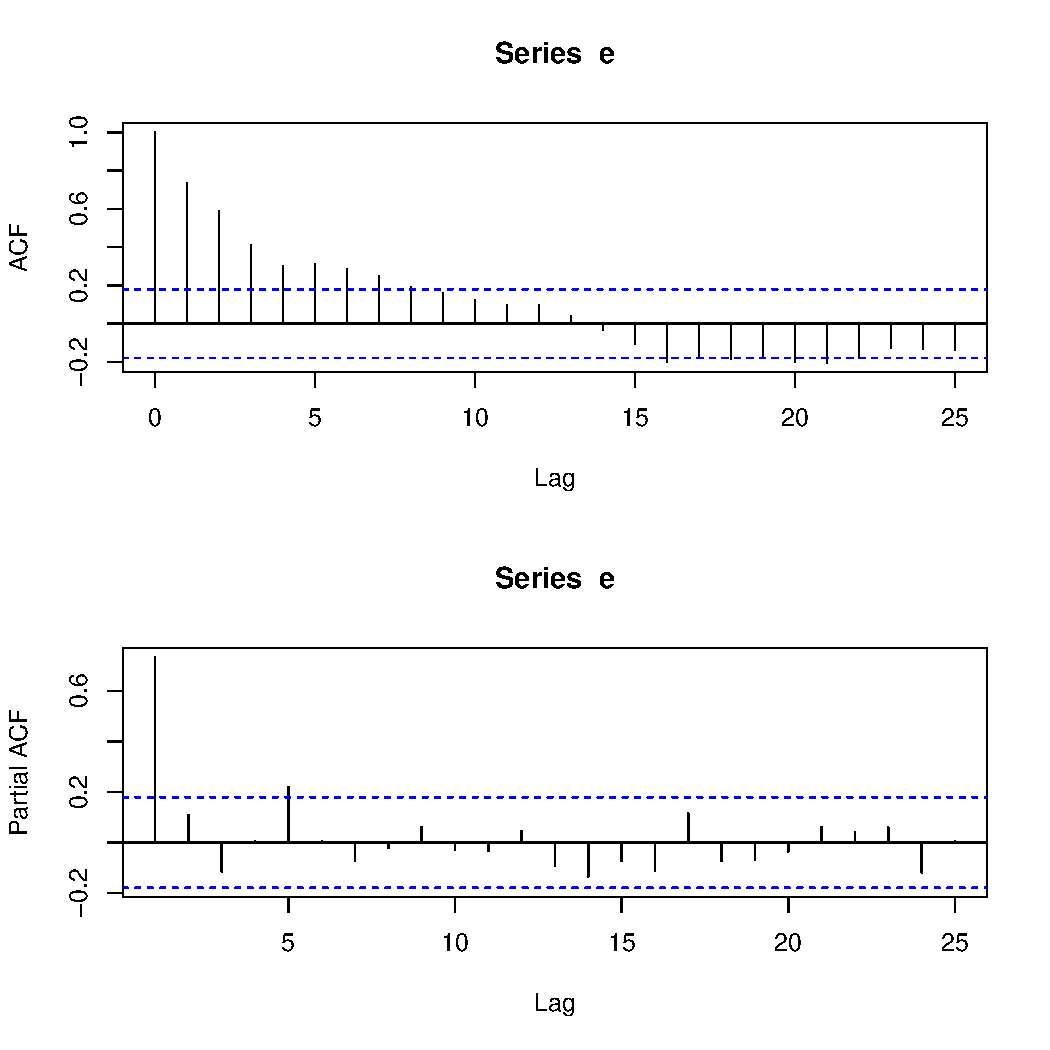
\includegraphics[width=0.6\textwidth]{figs/problem_8/acf_and_pacf.pdf}
    		\caption{ACF and PACF of regression residuals using monthly dummy variables.}
    		\label{fig:acf_and_pacf}
	\end{figure}
		
		\item We improve upon the ARIMA$(3,0,0)\text{x}(1,1,0)_{12}$ model from class by fitting an \\
		ARIMA$(1,0,1)\text{x}(1,1,0)_{12}$. The original model has AIC = -385.57 and BIC = -369.48 while the second model has smaller AIC and BIC values of AIC = -387.1 and BIC = -373.69. We also note that with the Box-Ljung test both models produce residuals that appear to have no significant autocorrelation. 
		
		\item	 We use both models to predict the next year and then compare these predictions with the actual time series values. The predictions and their associated 95\% confidence intervals are shown. To compare the prediction error the mean squared error was calculated for both models. The regression model performed better with an MSE of -633.4 while the SARIMA model had an MSE of 1804.8. This agrees with our AIC and BIC metrics. The regression model had a lower BIC at -397.40 while the SARIMA model had a BIC of -373.7. 
		
	\begin{figure}[H]
    		\centering
    		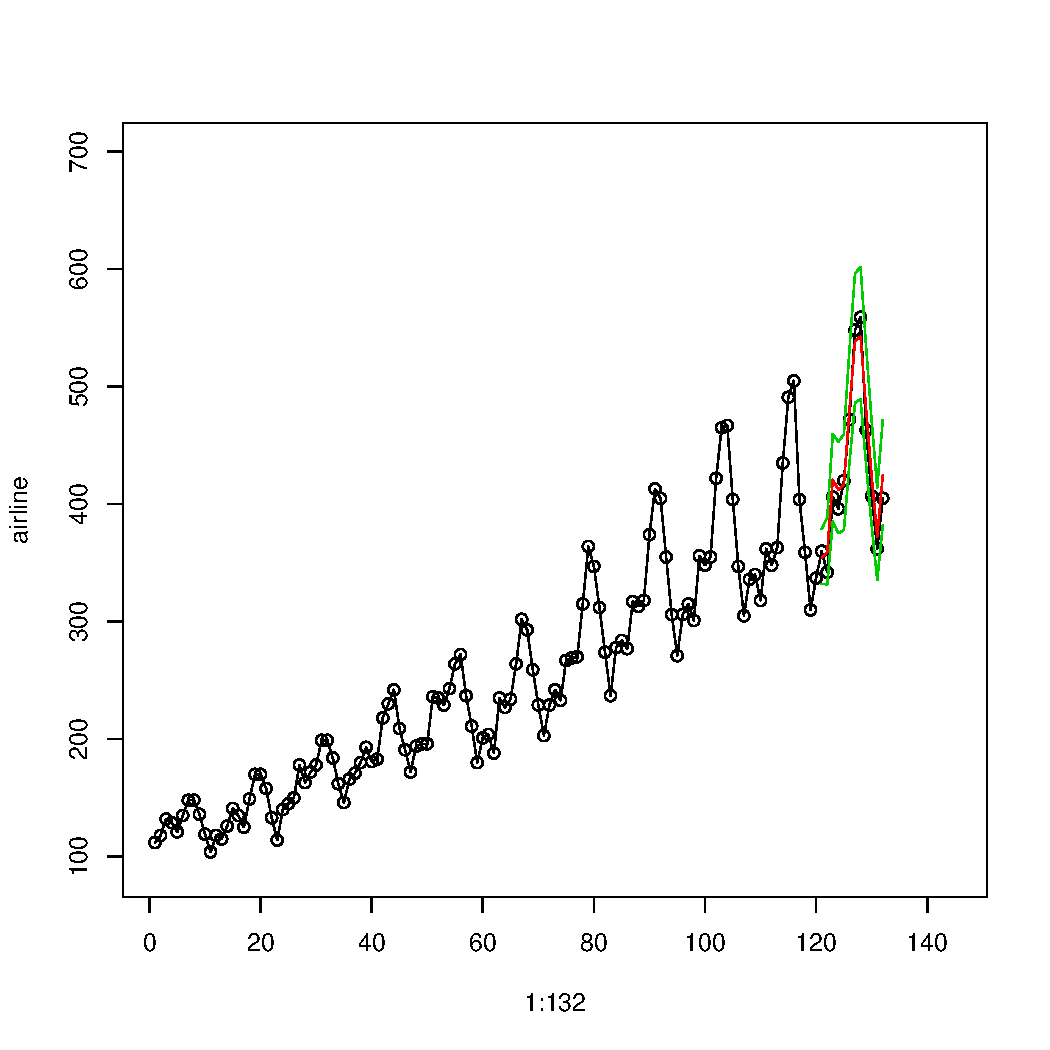
\includegraphics[width=0.8\textwidth]{figs/problem_8/reg_pred.pdf}
    		\caption{1 year ahead prediction using the AR(1) regression model.}
    		\label{fig:reg_pred}
	\end{figure}
	
	\begin{figure}[H]
    		\centering
    		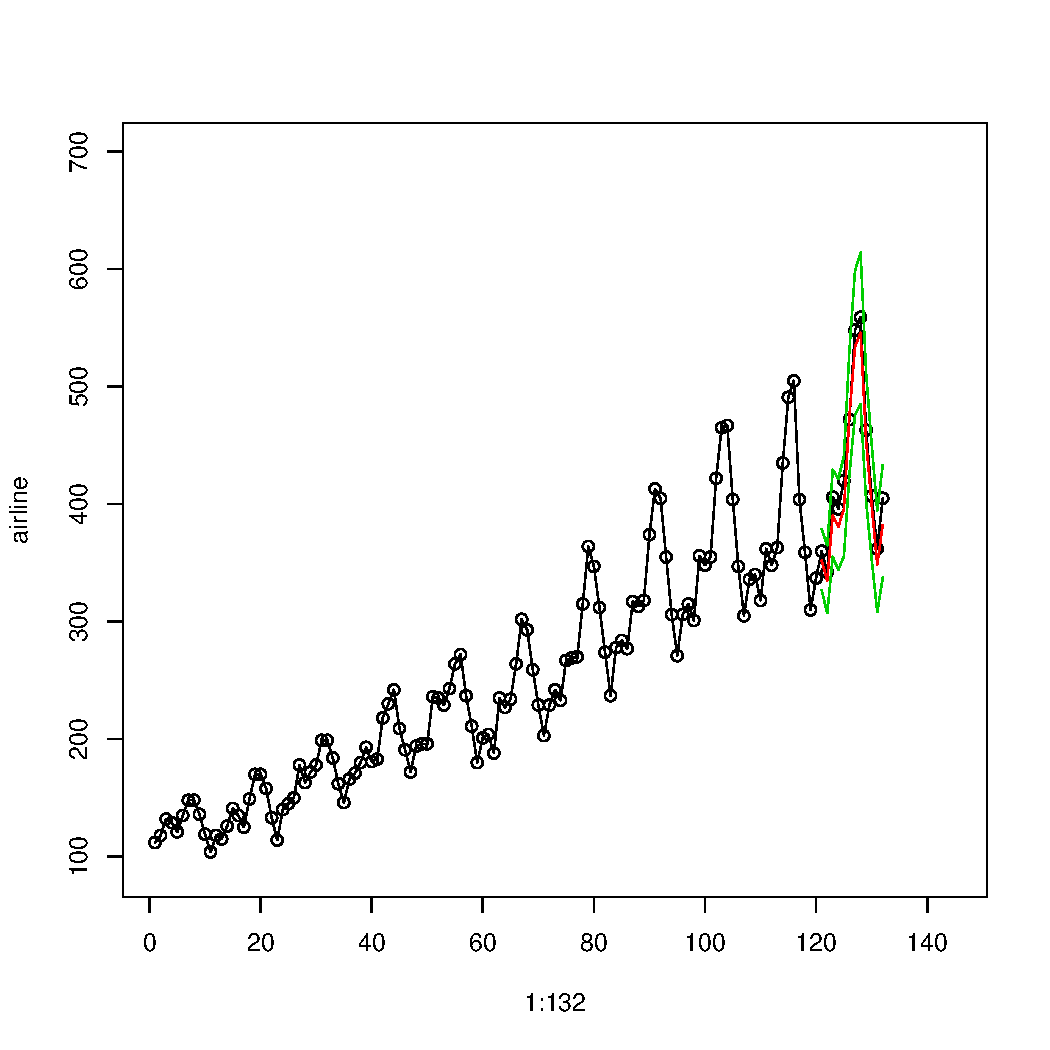
\includegraphics[width=0.8\textwidth]{figs/problem_8/sarima_pred.pdf}
    		\caption{a year ahead prediction using the ARIMA$(1,0,1)\text{x}(1,1,0)_{12}$ model.}
    		\label{fig:sarima_pred}
	\end{figure}
		
		
		\item	Our first model is given by
		
		\begin{equation*}
		Y_t = \beta_0 + \beta_1t + \beta_2M_1 + \beta_3M_2 + \beta_4M_3 + \beta_5M_4 + \beta_6M_5 + \beta_7M_6 + \beta_8M_7 + \beta_9M_8 + \beta_{10}M_9 + \beta_{11}M_10 + \epsilon_t.
		\end{equation*}
		
		\begin{equation*}
		\epsilon_t = \phi_1 X_{t-1} + Z_t,
		\end{equation*}
	
		\begin{equation*}
		\{Z_t\} \sim \text{WN}(0,\sigma^2).
		\end{equation*}
		
		Using this model to predict $Y_{121}$ we use the coefficients from the fit below. 
		
		\newpage
		
		\begin{lstlisting}
Coefficients:
         ar1     ar2  intercept   times      M1      M2      M3      M4      
      0.6825  0.1276     4.6981  0.0103  0.0124  0.0008  0.1363  0.0946  
s.e.  0.0918  0.0939     0.0318  0.0004  0.0117  0.0141  0.0158  0.0168  

       	  M5 	 M6      M7      M8      M9     M10      M11
      	0.0863  0.2113  0.3085  0.3003  0.1655  0.0245  -0.1174
s.e.  	0.0173  0.0175  0.0173  0.0166  0.0155  0.0137   0.0112

sigma^2 estimated as 0.001118:  log likelihood = 237,  aic = -442
		\end{lstlisting}
		
		\begin{equation*}
		Y_{121} = \beta_0 + \beta_1121 + \beta_2M_1 + \beta_3M_2 + \beta_4M_3 + \beta_5M_4 + \beta_6M_5 + \beta_7M_6 + \beta_8M_7 + \beta_9M_8 + \beta_{10}M_9 + \beta_{11}M_10 + \phi_1 X_{120} 
		\end{equation*}
			
	\end{enumerate}

	\end{solution}
	\pagebreak
	
	\end{document}
	